\documentclass[tikz,border=10pt]{standalone}

\begin{document}
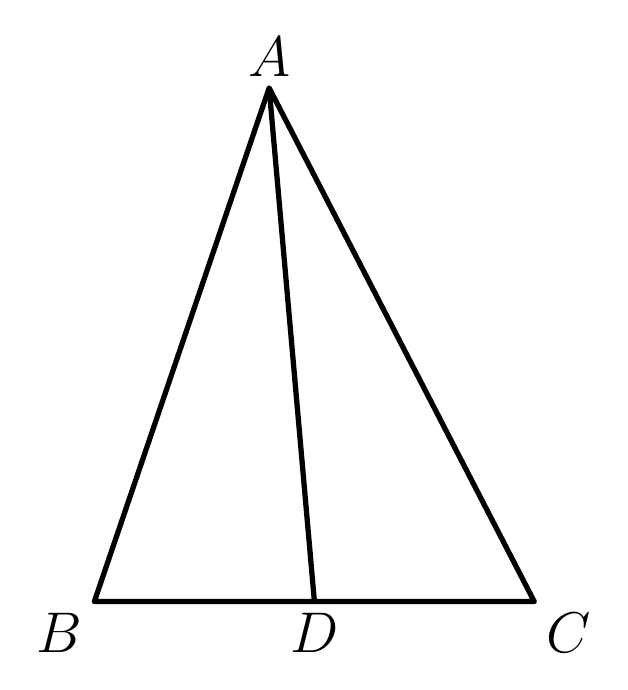
\begin{tikzpicture}[line width=1.9pt, line join=round]
\coordinate (A) at (-0.585,3.269);
\coordinate (B) at (-2.805,-3.254);
\coordinate (C) at (2.782,-3.254);
\coordinate (D) at (-0.010,-3.254);

  
  \draw (A) -- (B) -- (C) -- cycle;
  
  \draw (A) -- (D);
  
  \draw (B) -- (D) -- (C);
  
  \node[above, font=\fontsize{20}{24}\selectfont] at (A) {$A$};
  \node[below left, font=\fontsize{20}{24}\selectfont] at (B) {$B$};
  \node[below right, font=\fontsize{20}{24}\selectfont] at (C) {$C$};
  \node[below, font=\fontsize{20}{24}\selectfont] at (D) {$D$};
\end{tikzpicture}
\end{document}